\subsubsection{Task-adapted TabM}

% P1: Role of TabM and the two candidate input pools in Fig. 5(a).
TabM provides a parameter-efficient ensemble for hourly attenuation estimation by sharing hidden weight matrices across members while retaining member-specific transformations \cite{Gorishniy2025TabM}. Figure~\ref{fig:tabm_architecture}(a) shows its use with the meteorological inputs defined in Section~II. The full candidate pool contains 50 non-vertically-resolved base features and 106 pressure-level features; the base-pool comparison uses the same 50 base features alone. The base features comprise surface quantities, single-level diagnostics, and column-integrated variables. Each pressure-level feature represents one variable at a specified pressure level. At each RFE state, the retained $k$ features describe the observation hour; channel history, timestamps, and weather-category labels are excluded.

% P2: Preprocessing and replication of the same hourly input.
Missing values are filled with medians fitted on the training rows, and each input is standardized using the corresponding training mean and standard deviation. The attenuation target is also standardized for training. For hour $h$, let $\mathbf{x}_h\in\mathbb{R}^{k}$ denote the preprocessed retained input. This vector is replicated across $M=32$ members to form $\mathbf{X}_h\in\mathbb{R}^{M\times k}$, whose rows initially contain the same meteorological information.

% P3: Every matrix and operator in Fig. 5(b); the displayed equation moved here.
Figure~\ref{fig:tabm_architecture}(b) expands one hidden block. Its input $\mathbf{H}\in\mathbb{R}^{M\times d_{\mathrm{in}}}$ is scaled elementwise by the member-specific input adapter $\mathbf{R}$, multiplied by the shared matrix $\mathbf{W}\in\mathbb{R}^{d_{\mathrm{in}}\times d_{\mathrm{out}}}$, and scaled by the member-specific output adapter $\mathbf{S}$. Adding the member-specific bias $\mathbf{B}$, applying ReLU, and applying dropout gives
\begin{equation}
\mathbf{H}'=
\operatorname{Dropout}\!\left(
\operatorname{ReLU}\!\left(
\bigl[(\mathbf{H}\odot\mathbf{R})\mathbf{W}\bigr]\odot\mathbf{S}
+\mathbf{B}
\right)\right),
\label{eq:tabm_hidden_block}
\end{equation}
where $\odot$ denotes elementwise multiplication, $\mathbf{R}$ has the same dimensions as $\mathbf{H}$, and $\mathbf{S}$, $\mathbf{B}$, and $\mathbf{H}'$ have dimensions $M\times d_{\mathrm{out}}$. Rows correspond to ensemble members. Each block has its own $\mathbf{W}$, shared across its members. The network contains three blocks of output width 256, with dropout probability 0.1 during training; dropout is disabled for inference.

% P4: Member-specific heads, training-loss branch and inference-mean branch.
Each member has a separate scalar regression head, denoted by $h_m$ in Fig.~\ref{fig:tabm_architecture}(a), producing a standardized prediction $\widehat{z}_{m,h}$. All members are supervised against the same standardized attenuation target. The training loss is their squared error averaged uniformly over hours and members, as represented by the member-wise MSE branch. For inference, the predictions are averaged to obtain $\overline{z}_h$ and then transformed back to dB:
\begin{equation}
\widehat{A}_h
=\mu_A+\sigma_A\overline{z}_h
=\mu_A+\frac{\sigma_A}{M}\sum_{m=1}^{M}\widehat{z}_{m,h},
\label{eq:tabm_hourly_estimate}
\end{equation}
where $\mu_A$ and $\sigma_A$ are the target mean and standard deviation fitted on the training rows. The shared matrices provide the common nonlinear transformations, while the member-specific scales, biases, and heads distinguish the member predictions without duplicating every hidden weight matrix.

% P5: Training settings and link to the protocol explained in the following text.
The selected network is trained using AdamW with a learning rate of $2\times10^{-3}$, weight decay of 0.01, a batch size of 256, and 54 epochs. Meteorological input construction, training-fitted preprocessing, weather-aware validation, and independent feature-elimination paths adapt the original TabM architecture to this task. The validation criterion and RFE procedure are specified below, and Section~\ref{subsec:uk_frozen_hourly} describes evaluation with the local estimators frozen.

\begin{figure*}[t]
\centering
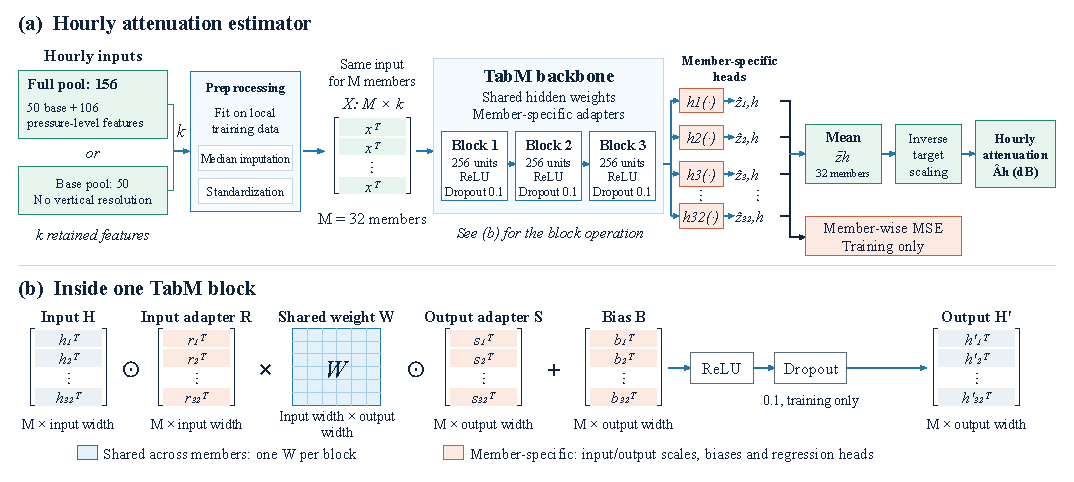
\includegraphics[width=\textwidth]{Fig05_TabM_Architecture_And_Protocol.pdf}
\caption{TabM architecture for hourly attenuation estimation. (a) Preprocessing, parallel member predictions, member-wise training loss, and averaged hourly output. (b) Operations within one hidden block. Blue denotes the hidden weight matrix shared across members; orange denotes member-specific scales, biases, and regression heads. The architecture follows TabM~\cite{Gorishniy2025TabM}. Here, $k$ is the retained input dimension and $M=32$ is the number of ensemble members.}
\label{fig:tabm_architecture}
\end{figure*}
